\documentclass[12pt]{article}
\usepackage{tikz}
\usetikzlibrary{patterns}

\begin{document}

Aquí comienza el documento en clase article.
\begin{figure}[h!]
\centering
\begin{tikzpicture}
    \draw (0,0) -- (2,2);
\end{tikzpicture}

\caption{Ejemplo 1}
\end{figure}

\begin{figure}[h!]
\centering
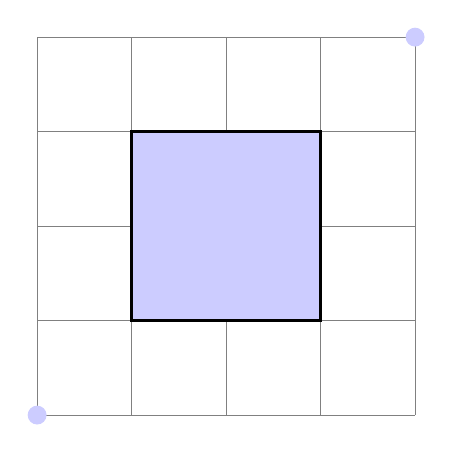
\begin{tikzpicture}[scale=1.2]
    \draw[help lines] (-2,-2) grid (2,2);
    \fill[blue!20] (-2,-2) circle (0.1);
    \fill[blue!20] (2,2) circle (0.1);
    \fill[blue!20] (0,0) circle (0.1);
    %\fill[blue!20] (0,0) circle (1.5);

    \begin{scope}
        \clip (-1,-1) rectangle (1,1);  % ventana de recorte

        % Todo lo siguiente queda recortado
        \fill[blue!20] (0,0) circle (1.5);
        %\draw[thick, blue] (0,0) circle (1.5);
    \end{scope}

    % Marco visible fuera del clip
    \draw[very thick] (-1,-1) rectangle (1,1);
\end{tikzpicture}
\caption{Ejemplo de clip en article}
\end{figure}



\begin{center}
    \begin{tikzpicture}

    % Línea fuera del scope
    \draw (0,0) -- (3,0);

    \begin{scope}[red, thick, rotate=20]
        \clip (0,0) rectangle (2,1);
        \draw (0,0) -- (3,0);  % rojo, grueso y rotado, pero recortado
    \end{scope}

    % Línea normal, sin rotación ni recorte
    \draw (0,0) -- (0,2);

\end{tikzpicture}
\end{center}

\begin{center}
    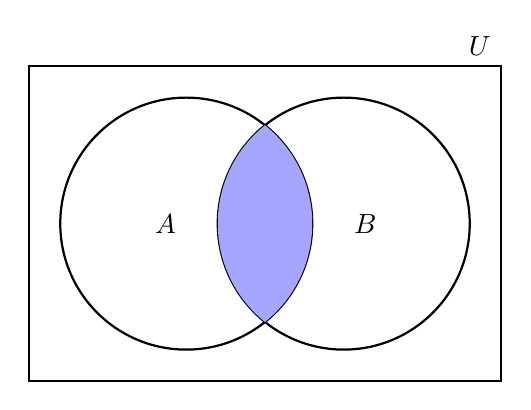
\begin{tikzpicture}[scale=1]
  % Marco (universo)
  \draw[thick] (-3,-2) rectangle (3,2) node[above left] {$U$};

  % Conjuntos A y B (contornos)
  \draw[thick] (-1,0) circle (1.6) node[left] {$A$};
  \draw[thick] ( 1,0) circle (1.6) node[right] {$B$};

  % Intersección A ∩ B usando doble clip
  \begin{scope}
    \clip (-1,0) circle (1.6);  % Clip a A
    \clip ( 1,0) circle (1.6);  % Clip a B -> intersección de ambos
    \fill[blue!35] (-3,-2) rectangle (3,2); % Sombreamos cualquier área grande
  \end{scope}
\end{tikzpicture}
\end{center}

\begin{center}
    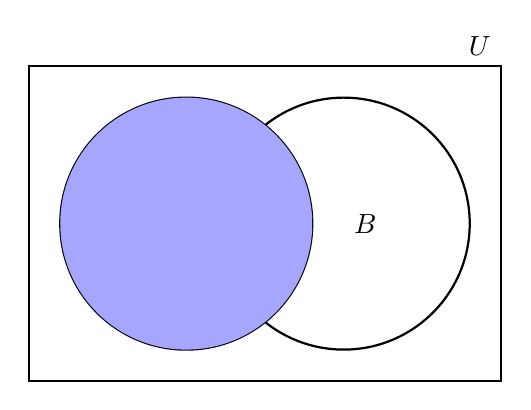
\begin{tikzpicture}[scale=1]
  % Marco (universo)
  \draw[thick] (-3,-2) rectangle (3,2) node[above left] {$U$};

  % Conjuntos A y B (contornos)
  \draw[thick] (-1,0) circle (1.6) node[left] {$A$};
  \draw[thick] ( 1,0) circle (1.6) node[right] {$B$};

  % Intersección A ∩ B usando doble clip
  \begin{scope}
    \clip (-1,0) circle (1.6);  % Clip a A
    %\clip ( 1,0) circle (1.6);  % Clip a B -> intersección de ambos
    \fill[blue!35] (-3,-2) rectangle (3,2); % Sombreamos cualquier área grande
  \end{scope}
\end{tikzpicture}
\end{center}


\begin{center}
    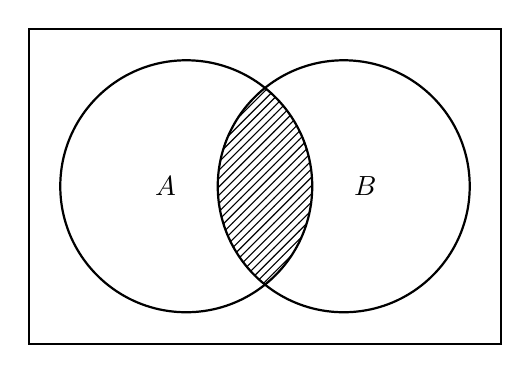
\begin{tikzpicture}[scale=1]
  \draw[thick] (-3,-2) rectangle (3,2);
  \draw[thick] (-1,0) circle (1.6) node[left] {$A$};
  \draw[thick] ( 1,0) circle (1.6) node[right] {$B$};

  \begin{scope}
    \clip (-1,0) circle (1.6);
    \clip ( 1,0) circle (1.6);
    \fill[pattern=north east lines] (-3,-2) rectangle (3,2);
  \end{scope}
\end{tikzpicture}
\end{center}

\begin{center}
    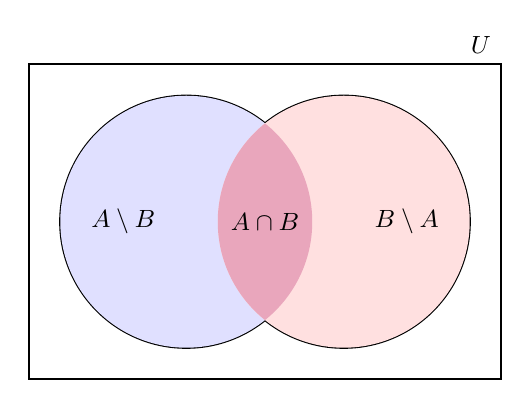
\begin{tikzpicture}[scale=1, every node/.style={font=\small}]
  % Universo
  \draw[thick] (-3,-2) rectangle (3,2) node[above left] {$U$};

  % Círculos
  \path (-1,0) coordinate (Acenter);
  \path ( 1,0) coordinate (Bcenter);
  \draw[thick] (Acenter) circle (1.6) node[left] {$A$};
  \draw[thick] (Bcenter) circle (1.6) node[right] {$B$};

  % A \ B
  \begin{scope}
    \clip (Acenter) circle (1.6);
    \fill[blue!12] (-3,-2) rectangle (3,2);
  \end{scope}

  % B \ A
  \begin{scope}
    \clip (Bcenter) circle (1.6);
    \fill[red!12] (-3,-2) rectangle (3,2);
  \end{scope}

  % Intersección A ∩ B (encima, más oscuro)
  \begin{scope}
    \clip (Acenter) circle (1.6);
    \clip (Bcenter) circle (1.6);
    \fill[purple!35] (-3,-2) rectangle (3,2);
  \end{scope}

  % Etiquetas en cada zona
  \node at (-1.8,0) {$A \setminus B$};
  \node at ( 0,  0) {$A \cap B$};
  \node at ( 1.8,0) {$B \setminus A$};
\end{tikzpicture}
\end{center}

\begin{center}
    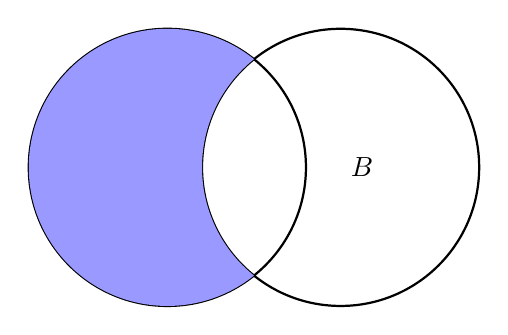
\begin{tikzpicture}[scale=1.1]
    % Contornos
    \draw[thick] (-1,0) circle (1.6) node[left] {$A$};
    \draw[thick] ( 1,0) circle (1.6) node[right] {$B$};

    % Para A - B:
    \begin{scope}
        % Clip al conjunto A
        \clip (-1,0) circle (1.6);

        % Ahora pintamos todo excepto B usando even odd rule
        \fill[blue!40, even odd rule]
            (-3,-3) rectangle (3,3)
            (1,0) circle (1.6);
    \end{scope}
\end{tikzpicture}
\end{center}


\begin{center}
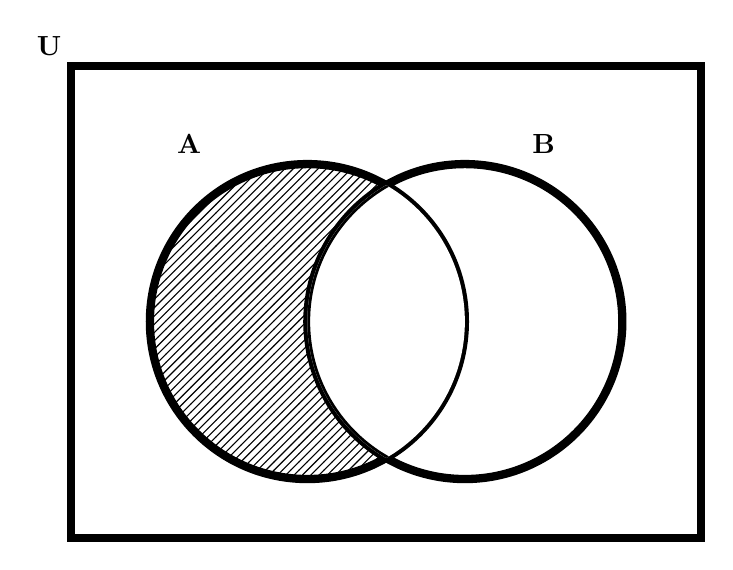
\begin{tikzpicture}
\draw[ line width = 3pt] (0,0) rectangle (8,6);
\draw[line width = 3pt] (3, 2.75) circle(2);
\draw[line width = 3pt] (5, 2.75) circle(2);
\begin{scope}
    \clip (3, 2.75) circle(2);
    \fill[pattern=north east lines] (0, 0) rectangle (8,6);
    \clip (5, 2.75) circle(2);
    \draw[line width = 2pt, fill = white] (5, 2.75) circle(2);
\end{scope}
\node at ( 1.5,  5) {$\mathbf{A}$};
\node at ( 6,  5) {$\mathbf{B}$};
\node at ( 0,  6)[above left] {$\mathbf{U}$};



\end{tikzpicture}
\end{center}


\begin{center}
    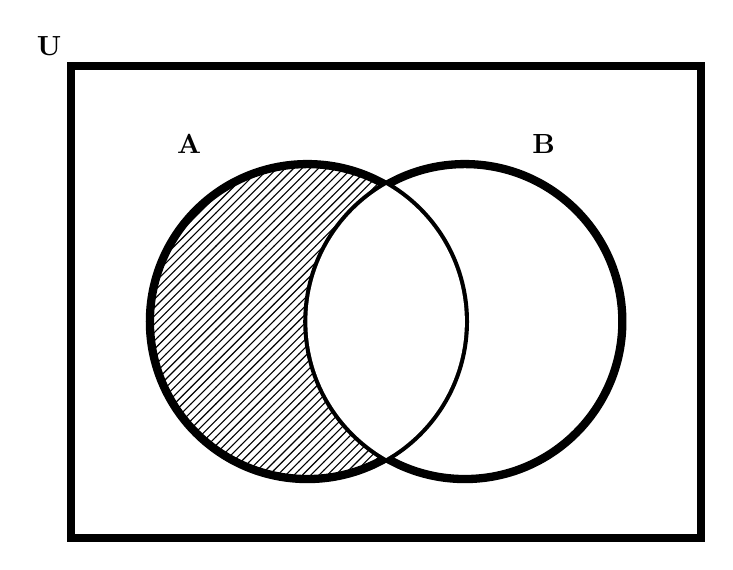
\begin{tikzpicture}

\draw[line width=3pt] (0,0) rectangle (8,6);

\draw[line width=3pt] (3,2.75) circle(2);
\draw[line width=3pt] (5,2.75) circle(2);

\begin{scope}

\clip (3,2.75) circle(2);
\fill[pattern=north east lines] (0,0) rectangle (8,6);

\fill[white] (5,2.75) circle(2);

\end{scope}

\node at (1.5,5) {$\mathbf{A}$};
\node at (6,5) {$\mathbf{B}$};
\node at (0,6)[above left] {$\mathbf{U}$};

\end{tikzpicture}
\end{center}


\begin{center}
    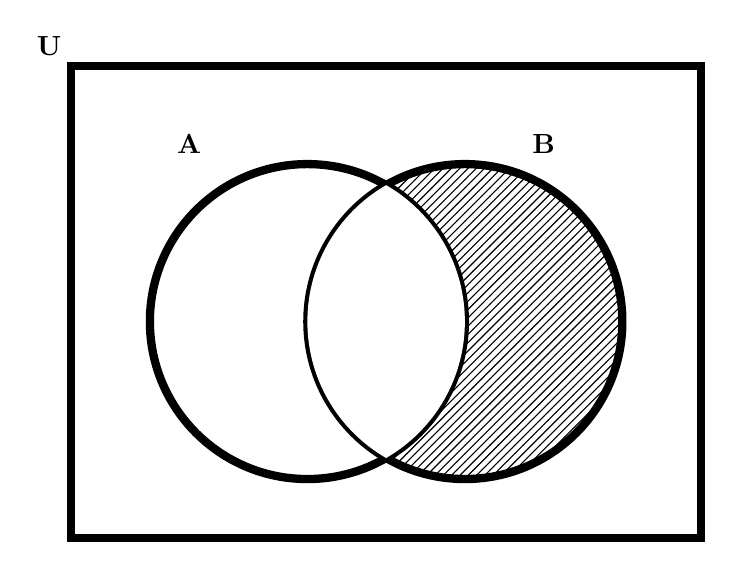
\begin{tikzpicture}

\draw[line width=3pt] (0,0) rectangle (8,6);

\draw[line width=3pt] (3,2.75) circle(2);
\draw[line width=3pt] (5,2.75) circle(2);

\begin{scope}

\clip (5,2.75) circle(2);
\fill[pattern=north east lines] (0,0) rectangle (8,6);

\fill[white] (3,2.75) circle(2);

\end{scope}

\node at (1.5,5) {$\mathbf{A}$};
\node at (6,5) {$\mathbf{B}$};
\node at (0,6)[above left] {$\mathbf{U}$};

\end{tikzpicture}
\end{center}


\begin{center}
    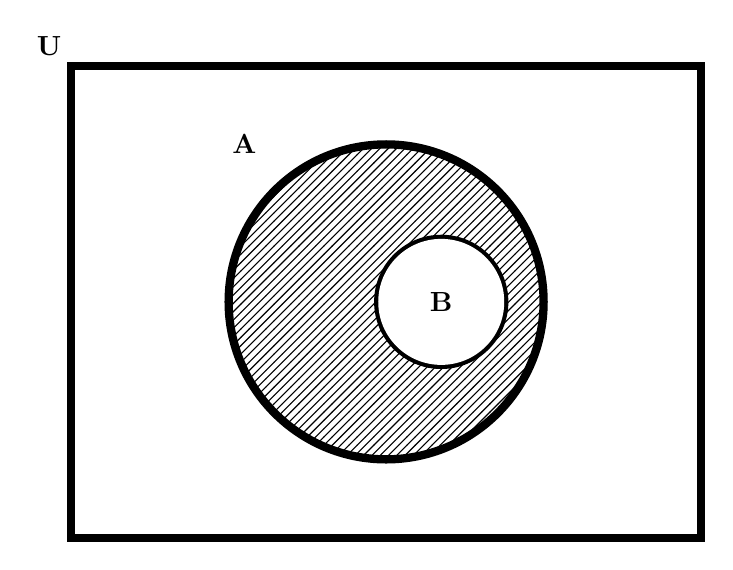
\begin{tikzpicture}

\draw[line width=3pt] (0,0) rectangle (8,6);

\draw[line width=3pt] (4,3) circle(2);      % Conjunto A
\draw[line width=3pt] (4.7,3) circle(0.8);  % Conjunto B dentro de A

\begin{scope}

\clip (4,3) circle(2); % recorte en A
\fill[pattern=north east lines] (0,0) rectangle (8,6);

\fill[white] (4.7,3) circle(0.8); % quitar B

\end{scope}

\node at (2.2,5) {$\mathbf{A}$};
\node at (4.7,3) {$\mathbf{B}$};
\node at (0,6)[above left] {$\mathbf{U}$};

\end{tikzpicture}
\end{center}


\begin{center}
    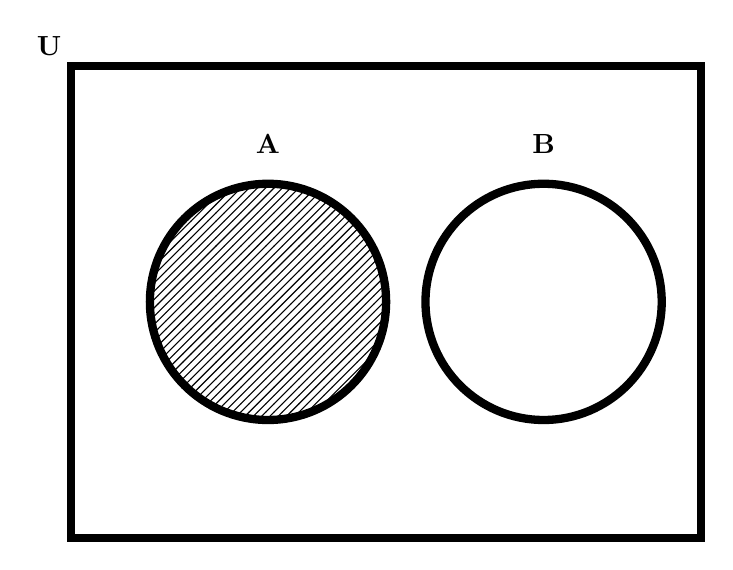
\begin{tikzpicture}

\draw[line width=3pt] (0,0) rectangle (8,6);

\draw[line width=3pt] (2.5,3) circle(1.5);  % A
\draw[line width=3pt] (6,3) circle(1.5);    % B (separado)

\begin{scope}

\clip (2.5,3) circle(1.5);
\fill[pattern=north east lines] (0,0) rectangle (8,6);

\end{scope}

\node at (2.5,5) {$\mathbf{A}$};
\node at (6,5) {$\mathbf{B}$};
\node at (0,6)[above left] {$\mathbf{U}$};

\end{tikzpicture}
\end{center}


\begin{center}
    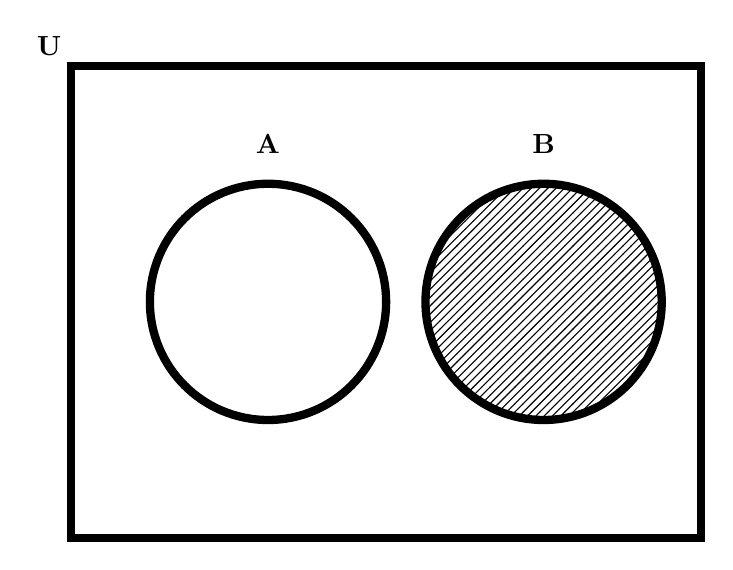
\begin{tikzpicture}

\draw[line width=3pt] (0,0) rectangle (8,6);

\draw[line width=3pt] (2.5,3) circle(1.5); % A
\draw[line width=3pt] (6,3) circle(1.5);   % B

\begin{scope}

\clip (6,3) circle(1.5);
\fill[pattern=north east lines] (0,0) rectangle (8,6);

\end{scope}

\node at (2.5,5) {$\mathbf{A}$};
\node at (6,5) {$\mathbf{B}$};
\node at (0,6)[above left] {$\mathbf{U}$};

\end{tikzpicture}
\end{center}



\begin{center}
    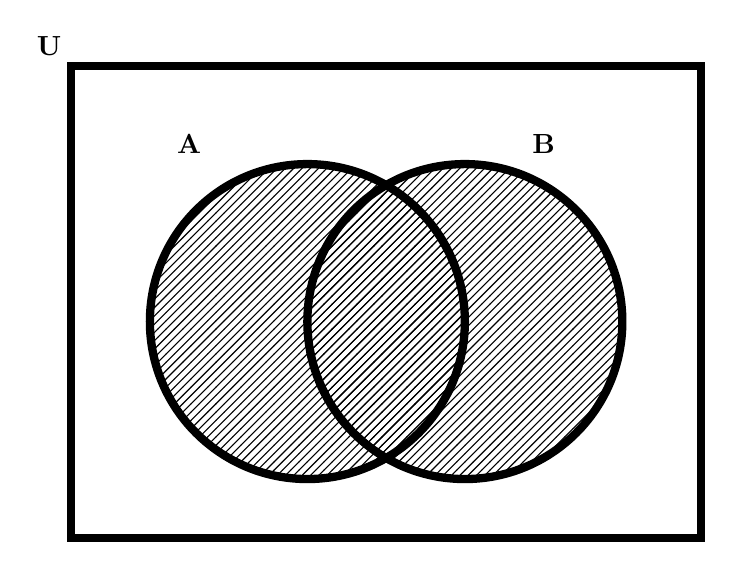
\begin{tikzpicture}

\draw[line width=3pt] (0,0) rectangle (8,6);

\draw[line width=3pt] (3,2.75) circle(2); % A
\draw[line width=3pt] (5,2.75) circle(2); % B

\begin{scope}

\clip (0,0) rectangle (8,6);
\fill[pattern=north east lines] (3,2.75) circle(2);
\fill[pattern=north east lines] (5,2.75) circle(2);

\end{scope}

\node at (1.5,5) {$\mathbf{A}$};
\node at (6,5) {$\mathbf{B}$};
\node at (0,6)[above left] {$\mathbf{U}$};

\end{tikzpicture}
\end{center}

\begin{center}
    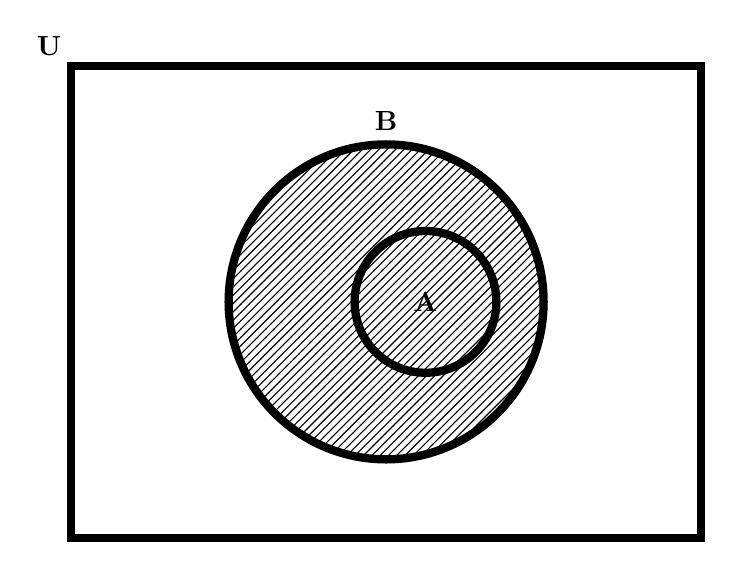
\begin{tikzpicture}

\draw[line width=3pt] (0,0) rectangle (8,6);

\draw[line width=3pt] (4,3) circle(2);      % B
\draw[line width=3pt] (4.5,3) circle(0.9);  % A dentro de B

\begin{scope}

\clip (4,3) circle(2);
\fill[pattern=north east lines] (0,0) rectangle (8,6);

\end{scope}

\node at (4.5,3) {$\mathbf{A}$};
\node at (4,5.3) {$\mathbf{B}$};
\node at (0,6)[above left] {$\mathbf{U}$};

\end{tikzpicture}
\end{center}

\begin{center}
    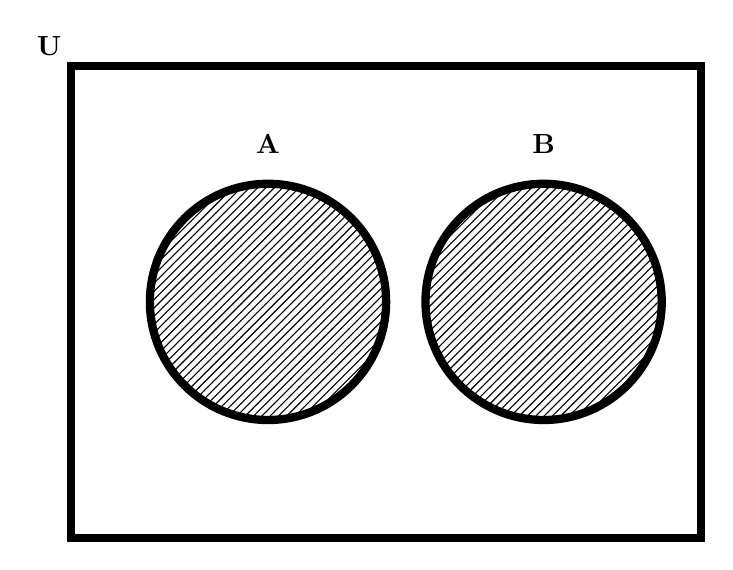
\begin{tikzpicture}

\draw[line width=3pt] (0,0) rectangle (8,6);

\draw[line width=3pt] (2.5,3) circle(1.5); % A
\draw[line width=3pt] (6,3) circle(1.5);   % B

\begin{scope}

\fill[pattern=north east lines] (2.5,3) circle(1.5);
\fill[pattern=north east lines] (6,3) circle(1.5);

\end{scope}

\node at (2.5,5) {$\mathbf{A}$};
\node at (6,5) {$\mathbf{B}$};
\node at (0,6)[above left] {$\mathbf{U}$};

\end{tikzpicture}
\end{center}


\begin{center}
    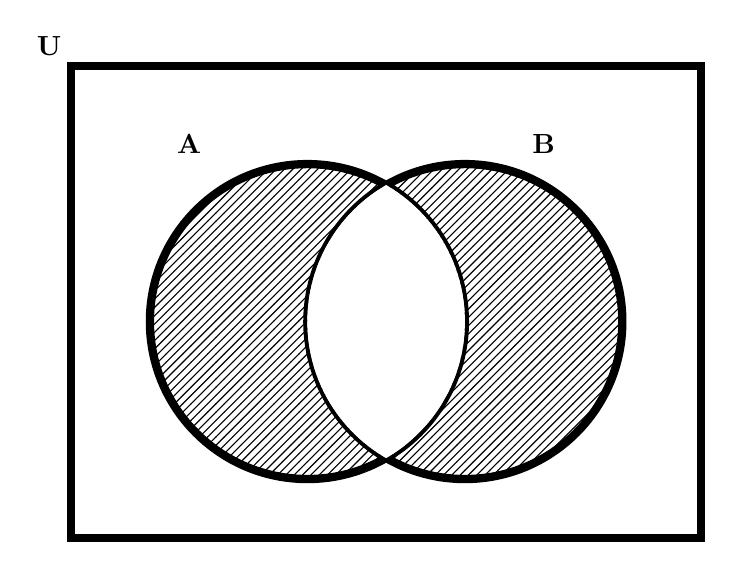
\begin{tikzpicture}

\draw[line width=3pt] (0,0) rectangle (8,6);

\draw[line width=3pt] (3,2.75) circle(2); % A
\draw[line width=3pt] (5,2.75) circle(2); % B

% Parte A-B
\begin{scope}
\clip (3,2.75) circle(2);
\fill[pattern=north east lines] (0,0) rectangle (8,6);
\fill[white] (5,2.75) circle(2);
\end{scope}

% Parte B-A
\begin{scope}
\clip (5,2.75) circle(2);
\fill[pattern=north east lines] (0,0) rectangle (8,6);
\fill[white] (3,2.75) circle(2);
\end{scope}

\node at (1.5,5) {$\mathbf{A}$};
\node at (6,5) {$\mathbf{B}$};
\node at (0,6)[above left] {$\mathbf{U}$};

\end{tikzpicture}
\end{center}

\begin{center}
    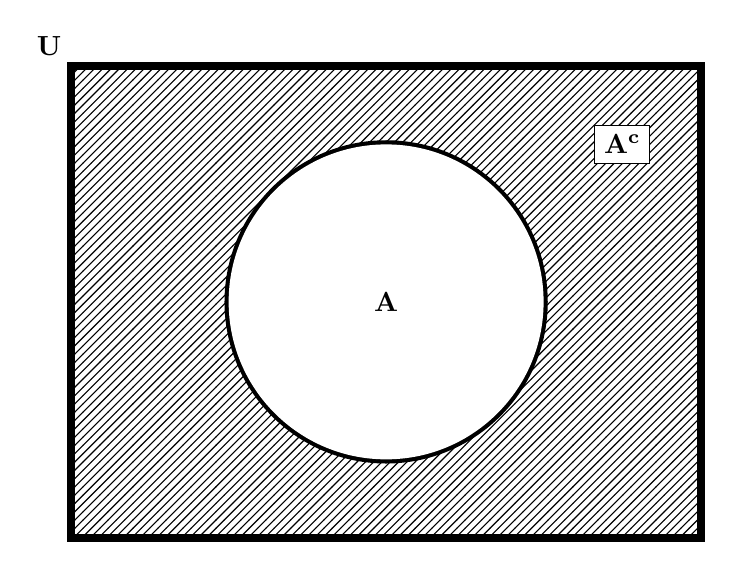
\begin{tikzpicture}

\draw[line width=3pt] (0,0) rectangle (8,6); % Universo
\draw[line width=3pt] (4,3) circle(2);       % Conjunto A

\begin{scope}

\clip (0,0) rectangle (8,6);
\fill[pattern=north east lines] (0,0) rectangle (8,6);
\fill[white] (4,3) circle(2);

\end{scope}

\node at (4,3) {$\mathbf{A}$};
\node at (0,6)[above left] {$\mathbf{U}$};
\node at (7,5) [draw, rectangle, fill=white] {$\mathbf{A^c}$};

\end{tikzpicture}
\end{center}
\end{document}

